%%%% Los documentos de LaTeX tienen dos partes
%%% Preámbulo, se cargan paqueterías y se definen parámetros de diseño
% Declarar una clase de documento
\documentclass[11pt,article]{memoir} % article, report, book

%%% Carga de paquetes
\usepackage[utf8]{inputenc} % para escribir con acentos en el archivo .tex
\usepackage[spanish,es-nodecimaldot]{babel} % para que escribamos en español

%% Para usar matemáticas
\usepackage{amscd} % crear diagramas conmutativos
\usepackage{amsfonts,amssymb,amsmath,amsthm}
\usepackage{mathrsfs} % letras matemáticas "elegantes"
\usepackage{bm} % negritas
\usepackage{bbm} % para poner la función indicadora
\usepackage{mathtools}

%%% Indispensables
\usepackage{graphicx}
\usepackage{subcaption}
\usepackage{hyperref}
\usepackage{enumitem}
\usepackage{multicol}
%\usepackage{geometry}

% No tan indispensables
\usepackage{tikz}
\usepackage{xcolor} % escribir con colores

\usepackage{macros}

% Crear comandos para escribir un poco menos
\newcommand{\edproba}{(\Omega, \mathscr F, \mathbb P)}

\title{Taller de R}
\author{Imanol}
\date{}

% Aquí acaba el preámbulo

%% El documento
\begin{document}
% Aquí va el documento   

\maketitle

\noindent Usualmente comienzo escribiendo sin sangría y uso \verb+\noindent+ para este fin. ¿Qué pasa si queremos escribir con cursiva? Para eso usamos \verb+\textit+ o \verb|\emph|, \textit{i.e.} \emph{esto debería salir en itálicas}.

Cada que queramos usar un comando tendremos que usar la notación que sigue: \verb|\comando{lo que tome como argumento}|

Algunos otros tipos de letra. \textbf{Negritas}. \textsc{mayúsculas pequeñas}. Otro tipo de letra es \texttt{teletype}.

Usamos \LaTeX{} porque es útil para escribir matemáticas. Por ejemplo, el teorema de Pitágoras nos dice que $ c^2 = a^2 + b^2 $, donde $c$ es la longitud de la hipotenusa y tanto $a$ como $b$ son las longitudes de los catetos de un triángulo rect\'angulo. 

Ya relacionado con probabilidad, tenemos un espacio de probabilidad, que es una terna $\edproba$ y tenemos el operador de esperanza $\mathbb E$. ¿Qué propiedades cumple la esperanza?

\begin{enumerate}
    \item Para v.a. $X$ y $Y$ tales que $\mathbb E[X]$, $\mathbb E[Y]$ y $\mathbb E[X+Y]$ existan se tiene que $\mathbb E [X+ Y] = \mathbb E [X] + \mathbb E[Y]$.
    \item Para una v.a. $X$ tal que $\mathbb E[X]$ exista, y para $\alpha \in \mathbb R$, $\mathbb E[\alpha X] = \alpha \mathbb E[X]$.
    \item Si $X \leq Y$ entonces $\EE[X] \leq \EE[Y]$.
\end{enumerate}

Yo para indicadoras uso $\mathbbm 1$, $\1$. Ahora escribamos algo un poco más elaborado, por ejemplo, la densidad de una variable aleatoria $X \sim U(0,1)$.
\[
f_X (x) = \mathbbm 1_{(0,1)}(x) = \begin{cases}
    1 & \text{si } x \in (0,1), \\
    0 & \text{si } x \notin (0,1).
\end{cases}
\]

De repente hacer dibujos es bueno para darnos a entender o para explicar nuestra intuición, entonces podemos agregar nuestros dibujos como en la figura \ref{cuadrito bonito}.

\begin{figure}
    \centering
    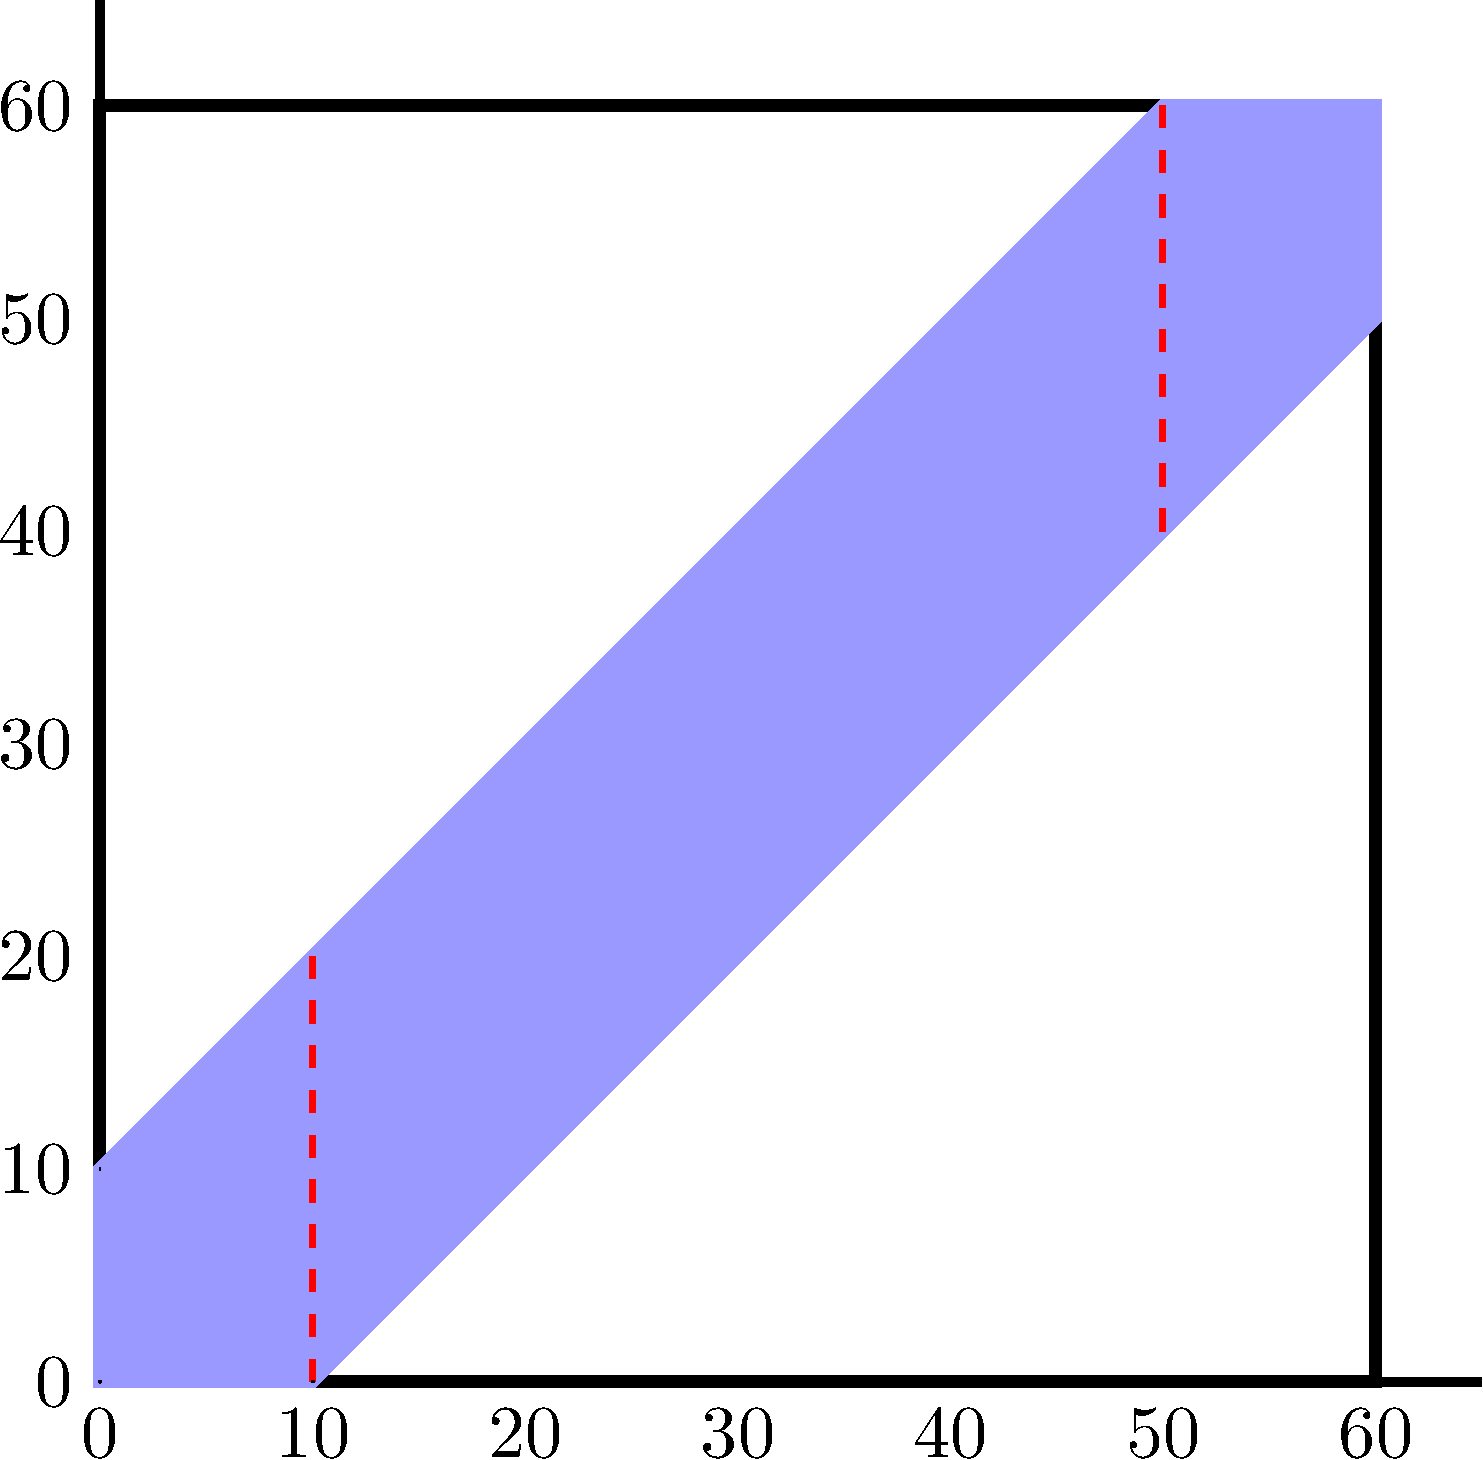
\includegraphics[width=0.5\textwidth,keepaspectratio]{cuadrito.pdf}
    \caption{Dibujito de un cuadrito. Fuente: hecha por mí.}
    \label{cuadrito bonito}
\end{figure}

Para evitar escribir ecuaciones en un solo renglón.

\begin{align*}
    \int_0^1 x dx & = \frac{1}{2} x^2 \bigg\vert_0^1 \\
    & = \frac{1}{2} - 0 \\
    & = \frac{1}{2}
\end{align*}

\end{document}